
 Let 
 \begin{align}
    \vec{A} = \myvec{4\\8\\10}, \vec{B} = \myvec{6\\10\\-8}.
 \end{align}
% Let $\vec{P}$ be the intersecting point of line $\vec{AB}$ and the YZ plane.
% Let the ratio in which $\vec{P}$ divides $\vec{AB}$ be $k:1$.\\
% Then,
and 
\begin{align}
%    \vec{P}-\vec{A} = k(\vec{B}-\vec{P})\\
    \vec{P}=\dfrac{\vec{A}+k\vec{B}}{k+1} \label{aug/2/19/eq}
\end{align}
Let the equation of the YZ plane be
\begin{align}
    \vec{n}^\top\vec{x}=d
\end{align}
Since $\vec{P}$ lies on YZ plane,
\begin{align}
    \vec{n}^\top\vec{P}&=d\\
    \implies \vec{n}^\top\left(\dfrac{\vec{A}+k\vec{B}}{k+1}\right)&=d\\
    %\implies \vec{n}^\top\vec{A}+k\vec{n}^\top\vec{B}=d(k+1)\\
    \implies k&=\dfrac{d-\vec{n}^\top\vec{A}}{\vec{n}^\top\vec{B}-d}
\end{align}
For YZ plane, $\vec{n}=\myvec{1\\0\\0}$ and $d=0$. So,
\begin{align}
    % &k=\dfrac{0-\myvec{1 & 0 & 0}\vec{A}}{\myvec{1 & 0 & 0}\vec{B}-0}\\
    % \implies &k=\dfrac{-\myvec{1 & 0 & 0}\myvec{4\\8\\10}}{\myvec{1 & 0 & 0}\myvec{6\\10\\-8}}\\
    % \implies &k=\dfrac{-4}{6}\\
 k=-2/3
\end{align}
%So, YZ plane divides line segment $\vec{AB}$ externally in the ratio 2:3.\\
Also, using \eqref{aug/2/19/eq}
\begin{align}
    \vec{P}&=\dfrac{\vec{A}-(2/3)\vec{B}}{(-2/3)+1}=3\vec{A}-2\vec{B}\\
    &=\myvec{0\\4\\46}
\end{align}
See Fig.      \ref{aug/2/19/plot}.
\begin{figure}[!hb]
    \centering
         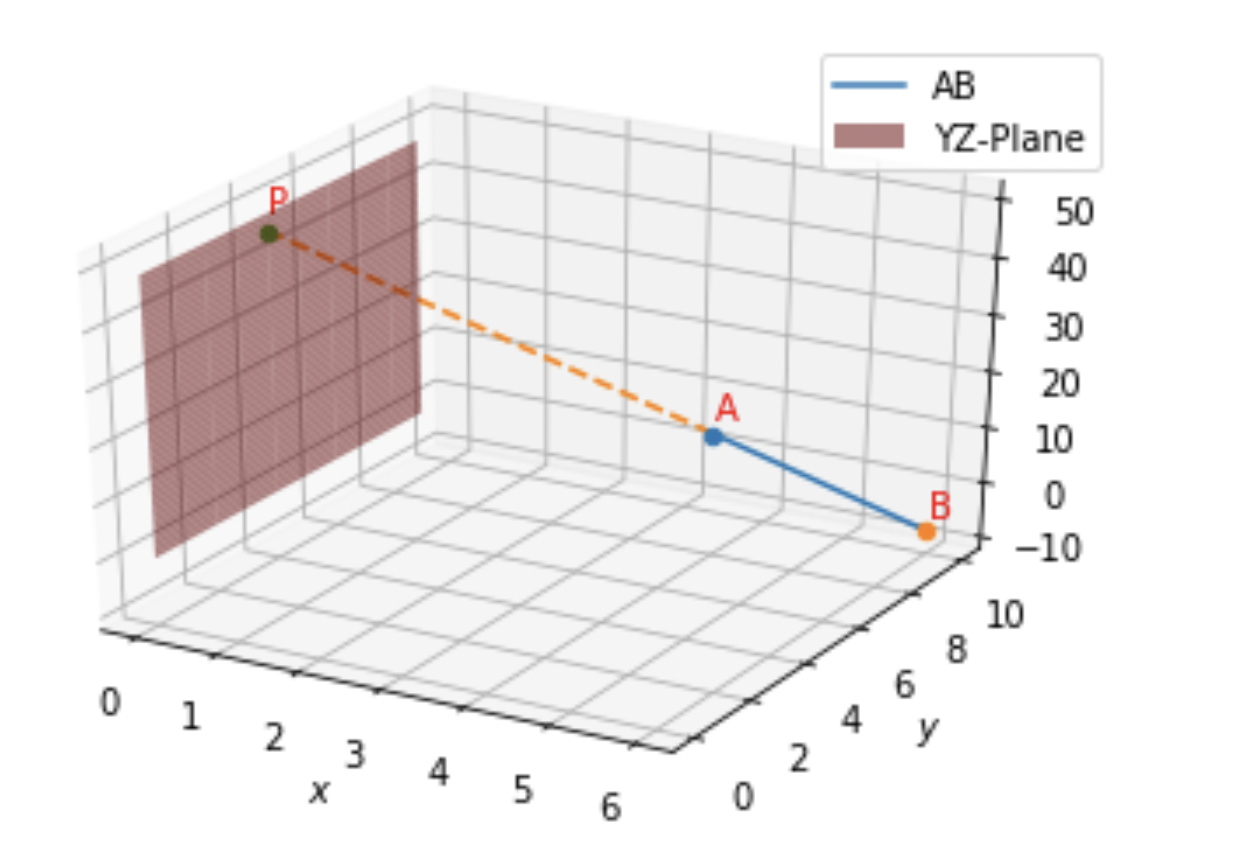
\includegraphics[width=\columnwidth]{solutions/aug/2/19/figures/figure.png}
         \caption{3D plot}
         \label{aug/2/19/plot}
\end{figure}

